\subsection{Особенности химического поведения электронодефицитных соединений, их связь с электронным строением.}

Рассмотрим соединения бора типа BX3 (рис. 1). В газовой фазе и в растворах такие молекулы плоские (в кристалле могут быть неплоские). Кроме ВН3, это всё мономерные
соединения. ВН3 координируется в диборан В2Н6. Вокруг атома бора находится 6 электронов, что не коррелирует с правилом инертного газа. Одна p-орбиталь бора остаётся пустой.
Молекулы такого типа называются электронодефицитными орбиталеизбыточными. Заместители у бора могут быть как одинаковые (галогенид-ионы, органические заместители,
гидроксил-ионы, водород), так и все разные.

Важным свойством рассматриваемых соединений является способность взаимодействовать с лигандами (какая-то молекула, способная предоставить электронную пару, или
несколько их). К лигандам можно отнести воду, простые эфиры, сульфиды, амины и т.д. Важно, что, к примеру, в аминах, связь разрывается не гомолитически, а гетеролитически, то
есть электронная пара остаётся у азота (рис. 2)

Интересно, что при взаимодействии BX3 и лиганда всегда образуется тетраэдрическая структура (рис. 3). Получается, что добавление лиганда не только ликвидирует
электронодефицитность молекулы, но и изменяет геометрию окружения атома бора. 

На рис. 4 приведена реакция BF3 с диэтиловым эфиром. Реакция необратима, и диэтиловый эфир из молекулы можно удалить только реакцией с другим лигандом. Температура
кипения такого продукта 101 градус, тогда как просто диэтиловый эфир - очень летучая и легкокипящая жидкость.

На рис. 5 приведена реакция BF3 с водой (в небольшом количестве, чтобы не допустить гидролиза). Наблюдается переход сначала от электронодефицитного соединения к
электронодостаточному, а затем от электронодостаточного к электроноизбыточному

На рис. 6 представлена схема взаимодействия BF3 с фторангидридом уксусной кислоты.

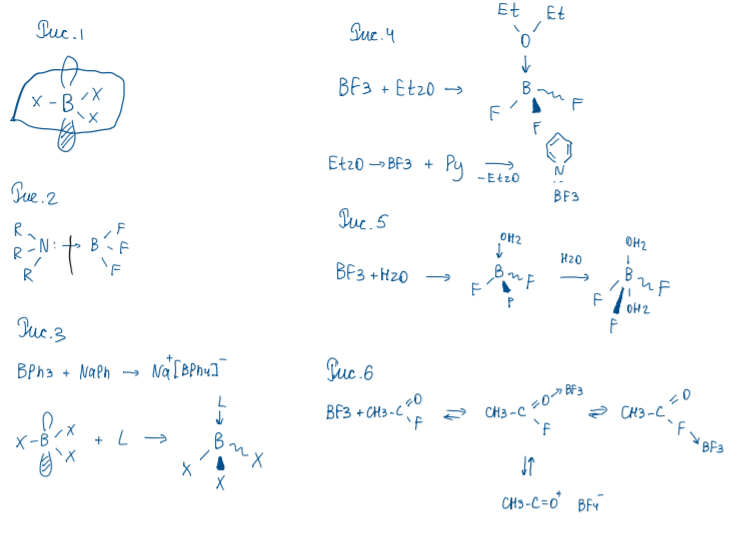
\includegraphics{images/16v1.png}

На рис. 7 представлена диаграмма МО BF3

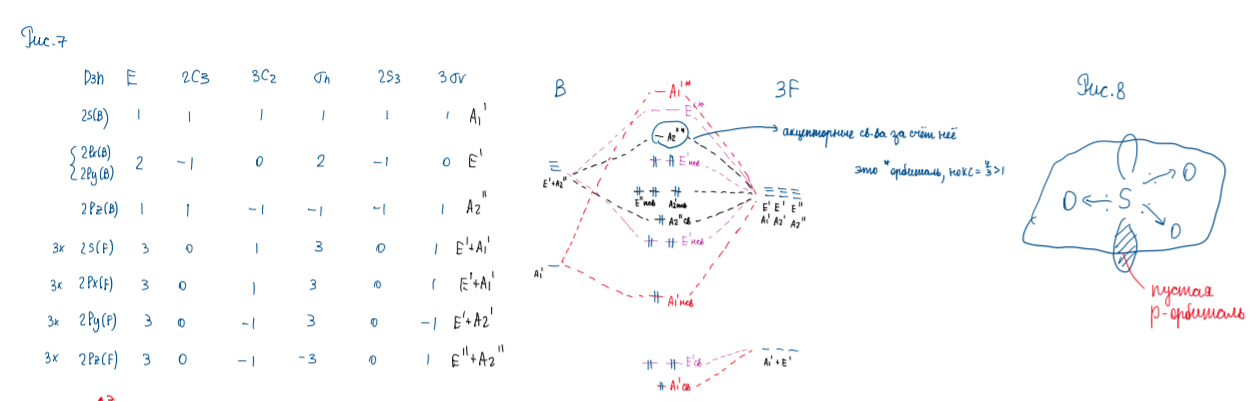
\includegraphics[scale=0.75]{images/16v2.png}

Помимо соединений 3А группы (короткопериодная таблица), хорошим примером электронодефицитного соединения является молекула SO3. В газовой фазе эта молекула имеет
плоское строение (рис. 8). В кристалле она не плоская, а составлена из тетраэдров, причем атомы кислорода одной молекулы выступают в качестве лиганда для другой молекулы
(рис. 9). Как и у бора в BF3, у серы имеется свободная орбиталь, что позволяет ей быть сильной кислотой Льюиса, то есть, акцептором электронной пары. 

На рис. 10 представлена реакция SO3 с пиридином. Получающееся соединение имеет пирамидальное строение, является сильнейшей кислотой Льюиса, а заместить пиридин
становится практически невозможно из-за сильной связи.

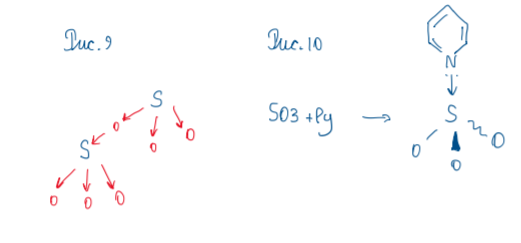
\includegraphics{images/16v3.png}

Заметим, что часто рисуют SO3 с тремя двойными связями к атомам кислорода. На самом деле, такое изображение не очень корректно, ведь у серы будет целых 12 электронов. Из
диаграммы МО (рис. 11) следует, что реально в связывании принимают только три орбитали серы, а одна р-орбиталь остается пустой. Взаимодействие же с ней р-орбиталей
кислорода второстепенно, им можно пренебречь. Получается, более правильным рисунком будет рис. 8, где есть три донорно-акцепторные связи, и от этого степень окисления серы
не изменится.

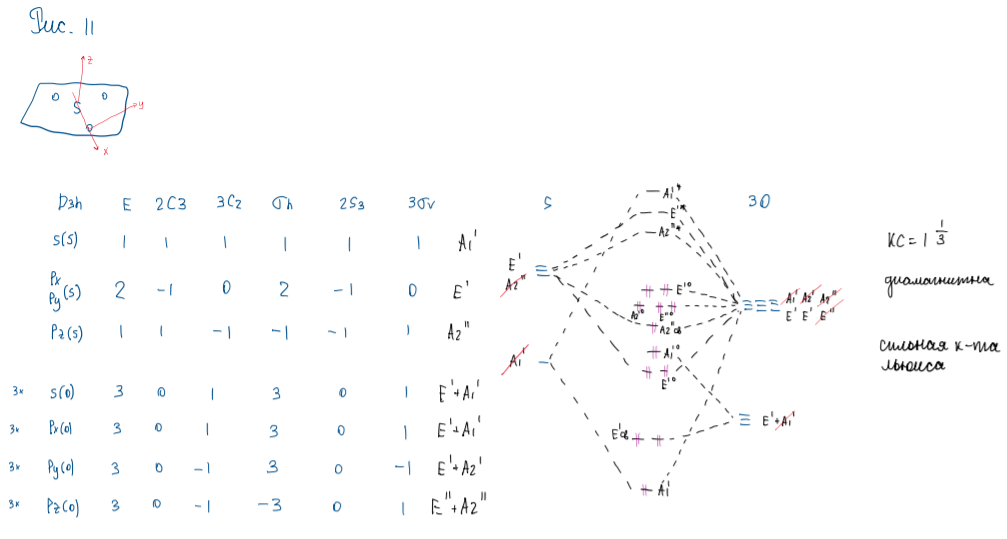
\includegraphics{images/16v4.png}